\documentclass{scrartcl}

% Kodierung dieser Datei angeben
\usepackage[utf8]{inputenc}

% Schönere Schriftart laden
\usepackage[T1]{fontenc}
\usepackage{lmodern}

% Deutsche Silbentrennung verwenden
\usepackage[ngerman]{babel}

% Bessere Unterstützung für PDF-Features
\usepackage[breaklinks=true]{hyperref}

\KOMAoptions{%
  % Absätze durch Abstände
  parskip=full,%
  % Satzspiegel berechnen lassen
  DIV=calc%
}

% Unterstützung für Grafiken
\usepackage{graphicx}

\begin{document}
  \begin{figure}
    \centering
    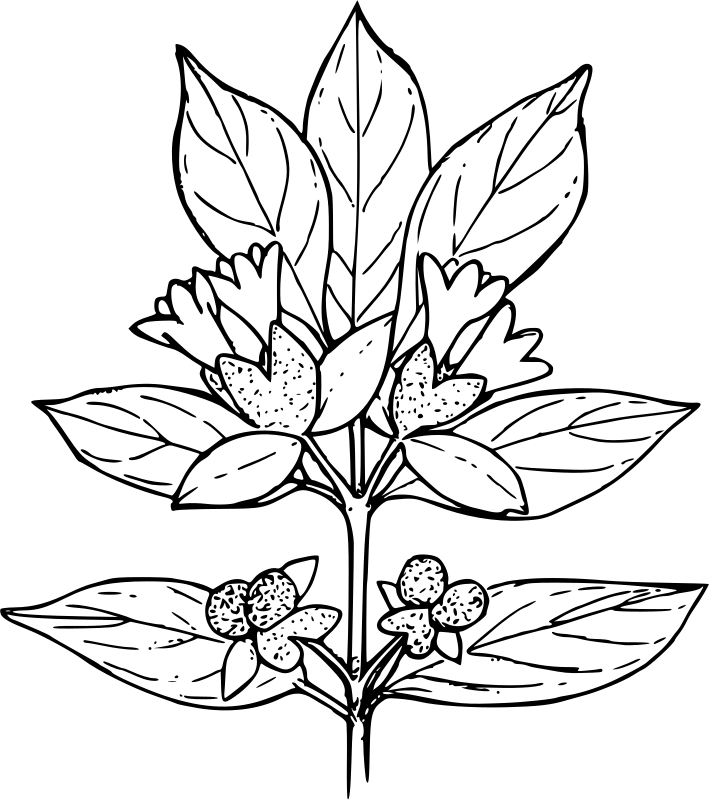
\includegraphics[width=6cm]{flower}
    \caption{Eine Blume. Diese Blume dient hier nur als ein
      Beispiel. In echten Dokumenten verwendet man am besten
      passendere Grafiken.}
    \label{fig:flower}
  \end{figure}

  In \autoref{fig:flower} ist eine Blume zu sehen. An dieser Blume
  kann man erkennen, wie eine Grafik in \LaTeX\ eingebunden werden
  kann.

  \begin{table}
    \centering
    \begin{tabular}{l|lr}
      \textbf{Jahr} & \textbf{Prozessor} &
          \textbf{MHz} \\
      \hline
      1975 & 6502 (C64) & 1 \\
      1985 & 80386 & 16 \\
      2005 & Pentium 4 & 2\,800 \\
      2030 & Phoenix 3 & 7\,320\,000
    \end{tabular}
    \caption{Eine Bildunterschrift sollte den gesamten Inhalt des
      Bildes zusammenfassen. Die meisten Leser betrachten als erstes
      die Bilder und müssen durch eine lange Bildunterschrift mit der
      Thematik der Arbeit vertraut gemacht werden.}
    \label{tab:prozessoren}
  \end{table}

  Die Geschwindigkeit der Prozessoren nimmt im Laufe der Zeit immer
  weiter zu. In \autoref{tab:prozessoren} ist die Takfrequenz in MHz
  für einige ausgewählte Modelle angegeben.

  Dieses Dokument muss mehrfach kompiliert werden, damit die Verweise
  funktionieren und folgenden Verzeichnisse korrekt erzeugt werden.

  \listoffigures
  \listoftables
\end{document}